\documentclass[newPxFont]{beamer}
%\documentclass[handout]{beamer} % Раздаточный материал (на слайдах всё сразу)
%\documentclass[aspectratio=169]{beamer} % Соотношение сторон


\usetheme{LTX}

%-=-=-=-=-=-=-=-=-=-=-=-=-=-=-=-=-=-=-=-=-=-=-=-=
%        LOADING PACKAGES
%-=-=-=-=-=-=-=-=-=-=-=-=-=-=-=-=-=-=-=-=-=-=-=-=
\usepackage[T2A]{fontenc}			% кодировка
\usepackage[utf8]{inputenc}			% кодировка исходного текста
\usepackage[english,russian]{babel}	% локализация и переносы


%%% Дополнительная работа с математикой
\usepackage{amsmath,amsfonts,amssymb,amsthm,mathtools} % AMS

%%% Работа с картинками
\usepackage{graphicx}  % Для вставки рисунков
\graphicspath{{images/}{images2/}}  % папки с картинками
\setlength\fboxsep{3pt} % Отступ рамки \fbox{} от рисунка
\setlength\fboxrule{1pt} % Толщина линий рамки \fbox{}
\usepackage{wrapfig} % Обтекание рисунков текстом

%%% Работа с таблицами
\usepackage{array,tabularx,tabulary,booktabs} % Дополнительная работа с таблицами
\usepackage{longtable}  % Длинные таблицы
\usepackage{multirow} % Слияние строк в таблице

%%% Программирование
\usepackage{etoolbox} % логические операторы

%%% Другие пакеты
\usepackage{multicol} % Несколько колонок

%%% Картинки
\usepackage{tikz} % Работа с графикой
\usepackage{pgfplots}
\usepackage{pgfplotstable}


\usepackage{xcolor}
\usepackage{hyperref}
\usepackage{verbatim}
\usepackage{fancyvrb}
\usepackage{mdframed}

\usepackage{chronology}

\renewcommand{\event}[3][e]{%
  \pgfmathsetlength\xstop{(#2-\theyearstart)*\unit}%
  \ifx #1e%
    \draw[fill=black,draw=none,opacity=0.5]%
      (\xstop, 0) circle (.2\unit)%
      node[opacity=1,rotate=45,right=.2\unit] {#3};%
  \else%
    \pgfmathsetlength\xstart{(#1-\theyearstart)*\unit}%
    \draw[fill=black,draw=none,opacity=0.5,rounded corners=.1\unit]%
      (\xstart,-.1\unit) rectangle%
      node[opacity=1,rotate=45,right=.2\unit] {#3} (\xstop,.1\unit);%
  \fi}%

\title{Уютный факультатив по \LaTeX}
\subtitle{Введение в \LaTeX}
\date{\today}

\begin{document}

 \maketitle
 

\begin{frame}

\end{frame} 


\begin{frame}

\end{frame}

\begin{frame}

\end{frame} 


\begin{frame}

\end{frame}

\begin{frame}

\end{frame} 


\begin{frame}

\end{frame}


\section{Markdown}

\begin{frame}
Что такое \LaTeX? \LaTeX{} - это разметка. Мы командами размечаем в какой части документа что нужно сделать. Существуют и другие разметки. Например, HTML, Markdown и т.п.
\end{frame}


\begin{frame}
\begin{center}

\includegraphics[width=0.6\linewidth]{md.png}
\end{center}
\begin{itemize}
\item Markdown - очень простая разметка для создания очень простых документов
\item К использованию Markdown можно переходить в R и в Python
\end{itemize}

%Например, я писал в Markdown свой блог о ЦМФ! 
\end{frame}

%Показываю синтаксис по ссылке из репозитория
 
\begin{frame}{Мемы}
\begin{center}
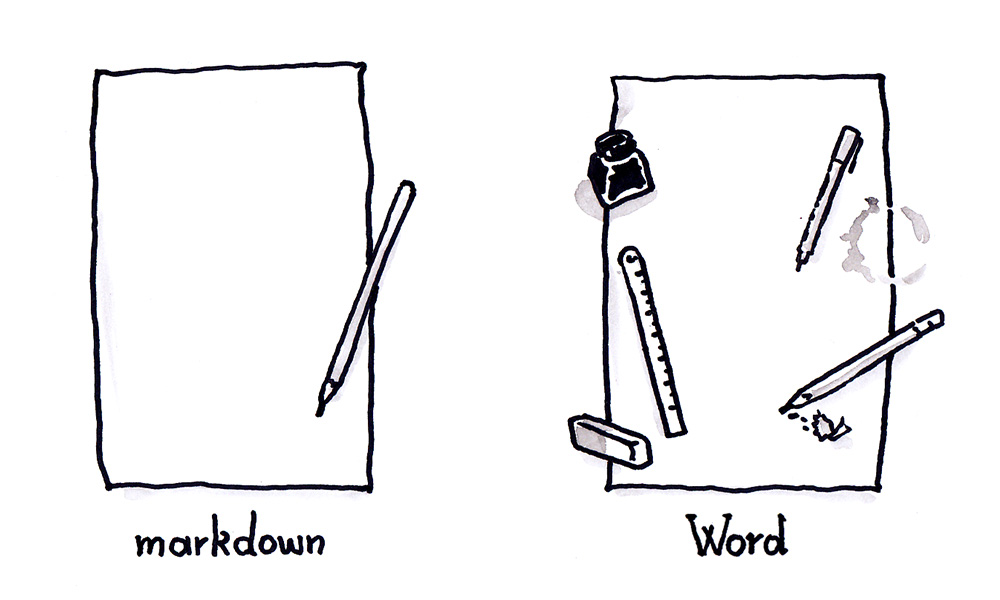
\includegraphics[width=0.6\linewidth]{mdwd.jpg}
\end{center}
\end{frame}


\begin{frame}[fragile]
\end{frame}

\end{document}